%%
%% This is file `sample-manuscript.tex',
%% generated with the docstrip utility.
%%
%% The original source files were:
%%
%% samples.dtx  (with options: `manuscript')
%% 
%% IMPORTANT NOTICE:
%% 
%% For the copyright see the source file.
%% 
%% Any modified versions of this file must be renamed
%% with new filenames distinct from sample-manuscript.tex.
%% 
%% For distribution of the original source see the terms
%% for copying and modification in the file samples.dtx.
%% 
%% This generated file may be distributed as long as the
%% original source files, as listed above, are part of the
%% same distribution. (The sources need not necessarily be
%% in the same archive or directory.)
%%
%% The first command in your LaTeX source must be the \documentclass command.
%%%% Small single column format, used for CIE, CSUR, DTRAP, JACM, JDIQ, JEA, JERIC, JETC, PACMCGIT, TAAS, TACCESS, TACO, TALG, TALLIP (formerly TALIP), TCPS, TDSCI, TEAC, TECS, TELO, THRI, TIIS, TIOT, TISSEC, TIST, TKDD, TMIS, TOCE, TOCHI, TOCL, TOCS, TOCT, TODAES, TODS, TOIS, TOIT, TOMACS, TOMM (formerly TOMCCAP), TOMPECS, TOMS, TOPC, TOPLAS, TOPS, TOS, TOSEM, TOSN, TQC, TRETS, TSAS, TSC, TSLP, TWEB.
% \documentclass[acmsmall]{acmart}

%%%% Large single column format, used for IMWUT, JOCCH, PACMPL, POMACS, TAP, PACMHCI
% \documentclass[acmlarge,screen]{acmart}

%%%% Large double column format, used for TOG
% \documentclass[acmtog, authorversion]{acmart}

%%%% Generic manuscript mode, required for submission and peer review
\documentclass[manuscript,screen,review]{acmart}
% review - Includes line numbers
% screen - Produces colored hyperlinks

%  The “lmodern” and “ltimes” packages should not be used, as they will override the built-in typeface families.

%%
%% \BibTeX command to typeset BibTeX logo in the docs
\AtBeginDocument{%
  \providecommand\BibTeX{{%
    \normalfont B\kern-0.5em{\scshape i\kern-0.25em b}\kern-0.8em\TeX}}}

%% Rights management information.  This information is sent to you
%% when you complete the rights form.  These commands have SAMPLE
%% values in them; it is your responsibility as an author to replace
%% the commands and values with those provided to you when you
%% complete the rights form.
\setcopyright{acmcopyright}
\copyrightyear{2018}
\acmYear{2018}
\acmDOI{10.1145/1122445.1122456}

%% These commands are for a PROCEEDINGS abstract or paper.
\acmConference[Woodstock '18]{Woodstock '18: ACM Symposium on Neural
  Gaze Detection}{June 03--05, 2018}{Woodstock, NY}
\acmBooktitle{Woodstock '18: ACM Symposium on Neural Gaze Detection,
  June 03--05, 2018, Woodstock, NY}
\acmPrice{15.00}
\acmISBN{978-1-4503-XXXX-X/18/06}


%%
%% Submission ID.
%% Use this when submitting an article to a sponsored event. You'll
%% receive a unique submission ID from the organizers
%% of the event, and this ID should be used as the parameter to this command.
%%\acmSubmissionID{123-A56-BU3}

%%
%% The majority of ACM publications use numbered citations and
%% references.  The command \citestyle{authoryear} switches to the
%% "author year" style.
%%
%% If you are preparing content for an event
%% sponsored by ACM SIGGRAPH, you must use the "author year" style of
%% citations and references.
%% Uncommenting
%% the next command will enable that style.
%%\citestyle{acmauthoryear}

%%
%% end of the preamble, start of the body of the document source.
\begin{document}

%%
%% The "title" command has an optional parameter,
%% allowing the author to define a "short title" to be used in page headers.
\title{The Name of the Title is Hope}
% To define a short title, you can use: \title[short title]{full title}

%%
%% The "author" command and its associated commands are used to define
%% the authors and their affiliations.
%% Of note is the shared affiliation of the first two authors, and the
%% "authornote" and "authornotemark" commands
%% used to denote shared contribution to the research.
\author{Ben Trovato}
\authornote{Both authors contributed equally to this research.}
\email{trovato@corporation.com}
\orcid{1234-5678-9012}
\author{G.K.M. Tobin}
\authornotemark[1]
\email{webmaster@marysville-ohio.com}
\affiliation{%
  \institution{Institute for Clarity in Documentation}
  \streetaddress{P.O. Box 1212}
  \city{Dublin}
  \state{Ohio}
  \country{USA}
  \postcode{43017-6221}
}

\author{Lars Th{\o}rv{\"a}ld}
\affiliation{%
  \institution{The Th{\o}rv{\"a}ld Group}
  \streetaddress{1 Th{\o}rv{\"a}ld Circle}
  \city{Hekla}
  \country{Iceland}}
\email{larst@affiliation.org}

%%
%% By default, the full list of authors will be used in the page
%% headers. Often, this list is too long, and will overlap
%% other information printed in the page headers. This command allows
%% the author to define a more concise list
%% of authors' names for this purpose.
\renewcommand{\shortauthors}{Trovato and Tobin, et al.}

%%
%% The abstract is a short summary of the work to be presented in the
%% article.
\begin{abstract}
  A clear and well-documented \LaTeX\ document is presented as an
  article formatted for publication by ACM in a conference proceedings
  or journal publication. Based on the ``acmart'' document class, this
  article presents and explains many of the common variations, as well
  as many of the formatting elements an author may use in the
  preparation of the documentation of their work.
\end{abstract}

%%
%% The code below is generated by the tool at http://dl.acm.org/ccs.cfm.
%% Please copy and paste the code instead of the example below.
%%
\begin{CCSXML}
<ccs2012>
 <concept>
  <concept_id>10010520.10010553.10010562</concept_id>
  <concept_desc>Computer systems organization~Embedded systems</concept_desc>
  <concept_significance>500</concept_significance>
 </concept>
 <concept>
  <concept_id>10010520.10010575.10010755</concept_id>
  <concept_desc>Computer systems organization~Redundancy</concept_desc>
  <concept_significance>300</concept_significance>
 </concept>
 <concept>
  <concept_id>10010520.10010553.10010554</concept_id>
  <concept_desc>Computer systems organization~Robotics</concept_desc>
  <concept_significance>100</concept_significance>
 </concept>
 <concept>
  <concept_id>10003033.10003083.10003095</concept_id>
  <concept_desc>Networks~Network reliability</concept_desc>
  <concept_significance>100</concept_significance>
 </concept>
</ccs2012>
\end{CCSXML}

\ccsdesc[500]{Computer systems organization~Embedded systems}
\ccsdesc[300]{Computer systems organization~Redundancy}
\ccsdesc{Computer systems organization~Robotics}
\ccsdesc[100]{Networks~Network reliability}

%%
%% Keywords. The author(s) should pick words that accurately describe
%% the work being presented. Separate the keywords with commas.
\keywords{datasets, neural networks, gaze detection, text tagging}


%%
%% This command processes the author and affiliation and title
%% information and builds the first part of the formatted document.
\maketitle

\section{Introduction}

%The ACM Computing Classification System ---
%\url{https://www.acm.org/publications/class-2012} --- is a set of
%classifiers and concepts that describe the computing
%discipline. Authors can select entries from this classification
%system, via \url{https://dl.acm.org/ccs/ccs.cfm}, and generate the
%commands to be included in the \LaTeX\ source.

\section{Sectioning Commands}

% The ``\verb|acmart|'' document class includes the ``\verb|booktabs|'' package --- \url{https://ctan.org/pkg/booktabs} --- for preparing high-quality tables.

%\begin{table}
%  \caption{Frequency of Special Characters}
%  \label{tab:freq}
%  \begin{tabular}{ccl}
%    \toprule
%    Non-English or Math&Frequency&Comments\\
%    \midrule
%    \O & 1 in 1,000& For Swedish names\\
%    $\pi$ & 1 in 5& Common in math\\
%    \$ & 4 in 5 & Used in business\\
%    $\Psi^2_1$ & 1 in 40,000& Unexplained usage\\
%  \bottomrule
%\end{tabular}
%\end{table}

% The table* environment sets a wider table which takes up the whole width of the page's live area
%\begin{table*}
%  \caption{Some Typical Commands}
%  \label{tab:commands}
%  \begin{tabular}{ccl}
%    \toprule
%    Command &A Number & Comments\\
%    \midrule
%    \texttt{{\char'134}author} & 100& Author \\
%    \texttt{{\char'134}table}& 300 & For tables\\
%    \texttt{{\char'134}table*}& 400& For wider tables\\
%    \bottomrule
%  \end{tabular}
%\end{table*}

% Always use midrule to separate table header rows from data rows, and use it only for this purpose.

%%% Figures %%%

%The ``\verb|figure|'' environment should be used for figures. One or
%more images can be placed within a figure. If your figure contains
%third-party material, you must clearly identify it as such, as shown
%in the example below.
%\begin{figure}[h]
%  \centering
%  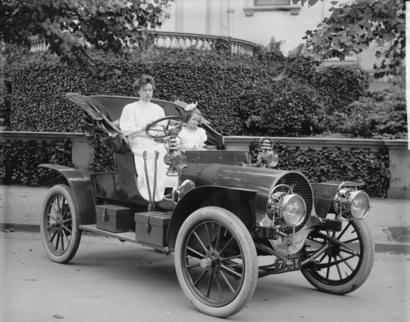
\includegraphics[width=\linewidth]{sample-franklin}
%  \caption{1907 Franklin Model D roadster. Photograph by Harris \&
%    Ewing, Inc. [Public domain], via Wikimedia
%    Commons. (\url{https://goo.gl/VLCRBB}).}
%  \Description{A woman and a girl in white dresses sit in an open car.}
%\end{figure}

% Every figure should also have a figure description unless it is purely decorative.
% A figure description must be unformatted plain text less than 2000 characters long (including spaces). Figure descriptions
% should not repeat the figure caption – their purpose is to capture important information that is not already provided in the caption.

%A ``teaser figure'' is an image, or set of images in one figure, that
%are placed after all author and affiliation information, and before
%the body of the article, spanning the page. If you wish to have such a
%figure in your article, place the command immediately before the
%\verb|\maketitle| command:
%\begin{verbatim}
%  \begin{teaserfigure}
%    \includegraphics[width=\textwidth]{sampleteaser}
%    \caption{figure caption}
%    \Description{figure description}
%  \end{teaserfigure}
%\end{verbatim}

\begin{verbatim}
  % \bibliographystyle{ACM-Reference-Format}
  % \bibliography{bibfile}
\end{verbatim}

%Identification of funding sources and other support, and thanks to individuals and groups that assisted in the research and the
%preparation of the work should be included in an acknowledgment section, which is placed just before the reference section in your
%document. Use the environment:

%\begin{acks}
%...
%\end{acks}

%%
%% The acknowledgments section is defined using the "acks" environment
%% (and NOT an unnumbered section). This ensures the proper
%% identification of the section in the article metadata, and the
%% consistent spelling of the heading.

%%
%% The next two lines define the bibliography style to be used, and
%% the bibliography file.
% \bibliographystyle{ACM-Reference-Format}
% \bibliography{sample-base}

%%
%% If your work has an appendix, this is the place to put it.
\appendix

\section{Research Methods}

\subsection{Part One}

TODO

\subsection{Part Two}

TODO

\section{Online Resources}

TODO

\end{document}
\endinput
%%
%% End of file `sample-manuscript.tex'.
